\chapter{Probability Spaces}\label{ch:probability-spaces}

\chapterinfo{STAT2003, STAT1301}{nothing}

% Sources: STAT2003 handwritten notes (pp. 1-7, 84); STAT2003 course notes, Chapter 1;
% STAT1301 course notes (2026), Sections 1.3-1.7.

The purpose of this chapter is to introduce the language of probability, which is an indispensable tool for understanding randomness. We describe random experiments by probability models, which consist of three building blocks: a sample space, a collection of events and a probability. We then show how to calculate probabilities by counting, and finish with conditional probability and independence.

% ==========================================================================
\section{Random experiments}\label{sec:random-experiments}
% ==========================================================================

A \emph{random experiment} is an experiment whose outcome cannot be determined in advance. Examples are:
\begin{enumerate}
  \item tossing a die;
  \item measuring the amount of rainfall in Brisbane in January;
  \item counting the number of calls arriving at a telephone exchange during a fixed time period;
  \item selecting a random sample of fifty people and observing the number of left-handers;
  \item choosing at random ten people and measuring their heights.
\end{enumerate}
The goal of probability is to understand the behaviour of random experiments by analysing the corresponding mathematical models. Mathematical models for random experiments are also the basis of statistics, where one fits an appropriate model to observed data.

\begin{example}[Coin tossing]\label{ex:coin-tossing-simulation}
The R program below simulates 100 tosses of a fair coin and plots the running average number of heads (\cref{fig:coin-running-average}). The average approaches $\tfrac12$, with a lot of random fluctuation. Similar results hold for a biased coin, with probability $p$ of heads.
\begin{rcode}
x <- sample(c(0, 1), size = 100, replace = TRUE)  # simulate coin tosses
y <- cumsum(x) / 1:100                            # running average
plot(y, type = "l")
\end{rcode}
Typical probability questions about this experiment are: what is the probability of $x$ heads in 100 tosses? How many heads would you expect to come up? A statistical analysis would instead start from observed data, for example the outcomes of 100 tosses, with $p$ unknown. Typical statistics questions are: is the coin fair? How can $p$ best be estimated from the data?
\end{example}

\begin{figure}[H]
\centering
\begin{tikzpicture}
\begin{axis}[bookplot, xmin=1, xmax=100, ymin=0, ymax=1, xlabel={Number of tosses $n$}, ylabel={Average number of heads}]
  \addplot[no marks, thin, color=thmcolor] table[x=n, y=r1] {figures/data/coin-running-average.dat};
  \addplot[no marks, thin, color=defcolor] table[x=n, y=r2] {figures/data/coin-running-average.dat};
  \addplot[no marks, thin, color=excolor] table[x=n, y=r3] {figures/data/coin-running-average.dat};
  \addplot[dashed, thin, domain=1:100] {0.5};
\end{axis}
\end{tikzpicture}
\caption{The average number of heads in $n$ tosses of a fair coin, $n = 1, \ldots, 100$, for three independent runs of the experiment.}
\label{fig:coin-running-average}
\end{figure}

% ==========================================================================
\section{Sample spaces and events}\label{sec:sample-spaces-events}
% ==========================================================================

We can usually specify the set of possible outcomes, even if we cannot predict which one will occur.

\begin{definition}[Sample space]\label{def:sample-space}
The \emph{sample space} $\Omega$ of a random experiment is the set of all possible outcomes of the experiment.
\end{definition}

For example, for the lifetime of a machine (in days) we can take $\Omega = \R^{+}$, the positive real numbers. For modelling purposes it is often easier to take the sample space larger than necessary: the actual lifetime of a machine would almost surely not span the entire positive real axis.

Often we are not interested in a single outcome, but in whether or not one of a group of outcomes occurs.

\begin{definition}[Event]\label{def:event}
An \emph{event} is a subset of the sample space. Events are denoted by capital letters $A, B, C, \ldots$. We say that event $A$ \emph{occurs} if the outcome of the experiment is one of the elements of $A$.
\end{definition}

Since events are sets, we can apply the usual set operations to them:
\begin{enumerate}
  \item $A \cup B$ ($A$ \emph{union} $B$) is the event that $A$ or $B$ or both occur;
  \item $A \cap B$ ($A$ \emph{intersection} $B$) is the event that $A$ and $B$ both occur;
  \item $A^c$ ($A$ \emph{complement}) is the event that $A$ does not occur;
  \item if $A \subseteq B$ ($A$ is a \emph{subset} of $B$), then event $A$ is said to \emph{imply} event $B$.
\end{enumerate}
The usual set laws (commutative, associative and distributive) apply. In particular, De Morgan's laws hold for any collection of events $\set{A_i}$:
\begin{equation}\label{eq:de-morgan}
  \Bigl(\bigcup_i A_i\Bigr)^c = \bigcap_i A_i^c, \qquad \Bigl(\bigcap_i A_i\Bigr)^c = \bigcup_i A_i^c.
\end{equation}
Two events $A$ and $B$ that have no outcomes in common, that is, $A \cap B = \emptyset$, are called \emph{disjoint} events. It is often useful to depict events in a Venn diagram, such as \cref{fig:venn-diagram}. In this diagram, $A \cap C = \emptyset$, so $A$ and $C$ are disjoint; and $(A \cap B^c) \cap (A^c \cap B) = \emptyset$, so $A \cap B^c$ and $A^c \cap B$ are disjoint.

\begin{figure}[H]
\centering
\begin{tikzpicture}
  \draw[thick] (-2.6,-1.6) rectangle (4.6,1.8);
  \node at (-2.3,1.5) {$\Omega$};
  \fill[thmcolor, opacity=0.15] (-0.5,0) circle (1.2);
  \fill[defcolor, opacity=0.15] (0.9,0) circle (1.2);
  \fill[excolor, opacity=0.15] (3.3,0) circle (0.9);
  \draw[thick] (-0.5,0) circle (1.2) (0.9,0) circle (1.2) (3.3,0) circle (0.9);
  \node at (-1.1,0) {$A \cap B^c$};
  \node at (0.2,0) {\small $A \cap B$};
  \node at (1.5,0) {$A^c \cap B$};
  \node at (-0.5,1.45) {$A$};
  \node at (0.9,1.45) {$B$};
  \node at (3.3,1.15) {$C$};
\end{tikzpicture}
\caption{A Venn diagram. Each set lies inside the sample space $\Omega$.}
\label{fig:venn-diagram}
\end{figure}

\begin{example}[Casting two dice]\label{ex:two-dice-events}
Suppose we cast two dice consecutively. The sample space is
\[
  \Omega = \set{(1,1), (1,2), \ldots, (1,6), (2,1), \ldots, (6,6)}.
\]
The event that the sum of the two dice is 10 or more is
\[
  \set{(4,6), (5,5), (5,6), (6,4), (6,5), (6,6)}.
\]
Let $A = \set{(6,1), \ldots, (6,6)}$ be the event that the first die is 6, and let $B = \set{(1,6), \ldots, (6,6)}$ be the event that the second die is 6. Then
\[
  A \cap B = \set{(6,1), \ldots, (6,6)} \cap \set{(1,6), \ldots, (6,6)} = \set{(6,6)}
\]
is the event that both dice are 6.
\end{example}

% ==========================================================================
\section{Probability}\label{sec:probability}
% ==========================================================================

The third ingredient in the model for a random experiment is the specification of the probability of the events. It tells us how likely it is that a particular event will occur.

\begin{definition}[Probability space]\label{def:probability-space}
A \emph{probability space} is a triple $(\Omega, \mathcal{F}, \Prob)$, where
\begin{itemize}
  \item $\Omega$ is the sample space;
  \item $\mathcal{F} \subseteq \powerset(\Omega)$ is the collection of events, where $\powerset(\Omega)$ is the set of all subsets of $\Omega$;
  \item $\Prob \colon \mathcal{F} \to [0, 1]$ is the probability measure.
\end{itemize}
\end{definition}

\begin{remark}
If $\Omega$ is infinite, $\mathcal{F}$ is infinite too. In that case $\mathcal{F}$ is taken to be a $\sigma$-algebra.
\end{remark}

\begin{definition}[Probability measure]\label{def:probability-measure}
A \emph{probability measure} $\Prob$ is a rule (function) which assigns a number to each event, and which satisfies the following axioms (Kolmogorov, 1933):
\begin{enumerate}[label=\textbf{Axiom \arabic*:}, leftmargin=*, widest=3]
  \item $\Prob(A) \ge 0$;
  \item $\Prob(\Omega) = 1$;
  \item for any sequence $A_1, A_2, \ldots$ of disjoint events,
  \begin{equation}\label{eq:sum-rule}
    \Prob\Bigl(\bigcup_i A_i\Bigr) = \sum_i \Prob(A_i).
  \end{equation}
\end{enumerate}
\end{definition}

Axiom 2 just states that the probability of the ``certain'' event $\Omega$ is 1. Property \eqref{eq:sum-rule} is the crucial property of a probability, and is sometimes referred to as the \emph{sum rule}. It states that if an event can happen in a number of different ways that cannot happen at the same time, then the probability of this event is simply the sum of the probabilities of the composing events.

Note that a probability rule $\Prob$ has exactly the same properties as the common ``area measure'': the total area of a union of non-overlapping triangles is the sum of the areas of the individual triangles. This is how you should interpret property \eqref{eq:sum-rule}. But instead of measuring areas, $\Prob$ measures probabilities.

\begin{example}[An unfair coin]\label{ex:unfair-coin}
A coin with heads worse than tails can be modelled by $\Omega = \set{H, T}$, $\mathcal{F} = \powerset(\Omega) = \set{\emptyset, \set{H}, \set{T}, \set{H, T}}$ and
\[
  \Prob(\set{H}) = 0.45, \qquad \Prob(\set{T}) = 0.55, \qquad \Prob(\emptyset) = 0, \qquad \Prob(\Omega) = 1.
\]
\end{example}

As a direct consequence of the axioms we have the following properties for $\Prob$.

\begin{theorem}[Properties of a probability measure]\label{thm:probability-properties}
Let $A$ and $B$ be events. Then
\begin{enumerate}
  \item $\Prob(\emptyset) = 0$;
  \item $A \subseteq B \implies \Prob(A) \le \Prob(B)$;
  \item $\Prob(A) \le 1$;
  \item $\Prob(A^c) = 1 - \Prob(A)$;
  \item $\Prob(A \cup B) = \Prob(A) + \Prob(B) - \Prob(A \cap B)$.
\end{enumerate}
\end{theorem}

\begin{proof}\leavevmode
\begin{enumerate}[leftmargin=*]
  \item[1.] Since $\Omega = \Omega \cup \emptyset$, we have, by the sum rule, $\Prob(\Omega) = \Prob(\Omega) + \Prob(\emptyset)$, and therefore, by the second axiom, $1 = 1 + \Prob(\emptyset)$, from which it follows that $\Prob(\emptyset) = 0$.
  \item[2.] If $A \subseteq B$, then $B = A \cup (B \cap A^c)$, where $A$ and $B \cap A^c$ are disjoint. Hence, by the sum rule, $\Prob(B) = \Prob(A) + \Prob(B \cap A^c)$, which is (by the first axiom) greater than or equal to $\Prob(A)$.
  \item[3.] This follows directly from property 2 and Axiom 2, since $A \subseteq \Omega$.
  \item[4.] $\Omega = A \cup A^c$, where $A$ and $A^c$ are disjoint. Hence, by the sum rule and Axiom 2, $1 = \Prob(\Omega) = \Prob(A) + \Prob(A^c)$, and thus $\Prob(A^c) = 1 - \Prob(A)$.
  \item[5.] Write $A \cup B$ as the disjoint union of $A$ and $B \cap A^c$. Then $\Prob(A \cup B) = \Prob(A) + \Prob(B \cap A^c)$. Also, $B = (A \cap B) \cup (B \cap A^c)$, so that $\Prob(B) = \Prob(A \cap B) + \Prob(B \cap A^c)$. Combining these two equations gives $\Prob(A \cup B) = \Prob(A) + \Prob(B) - \Prob(A \cap B)$. \qedhere
\end{enumerate}
\end{proof}

Property 5 extends to $n$ events.

\begin{theorem}[Inclusion--exclusion principle]\label{thm:inclusion-exclusion}
For events $E_1, \ldots, E_n$,
\begin{multline*}
  \Prob\Bigl(\bigcup_{i=1}^n E_i\Bigr) = \sum_i \Prob(E_i) - \sum_{i<j} \Prob(E_i \cap E_j) + \sum_{i<j<k} \Prob(E_i \cap E_j \cap E_k) - \cdots \\
  + (-1)^{n+1} \Prob(E_1 \cap \cdots \cap E_n).
\end{multline*}
In particular, $\Prob\bigl(\bigcup_i E_i\bigr) \le \sum_i \Prob(E_i)$.
\end{theorem}

We have now completed our model for a random experiment. It is up to the modeller to specify the sample space $\Omega$ and probability measure $\Prob$ which most closely describe the actual experiment.

\subsection{Discrete sample spaces}\label{sec:discrete-sample-spaces}

In many applications the sample space is countable, that is, $\Omega = \set{a_1, \ldots, a_n}$ or $\Omega = \set{a_1, a_2, \ldots}$. Such a sample space is called \emph{discrete}. The easiest way to specify a probability $\Prob$ on a discrete sample space is to specify first the probability $p_i$ of each elementary event $\set{a_i}$, and then to define
\[
  \Prob(A) = \sum_{i : a_i \in A} p_i \qquad \text{for all } A \subseteq \Omega.
\]
This idea is represented in \cref{fig:discrete-sample-space}. Each element $a_i$ of the sample space is assigned a probability weight $p_i$, represented by a dot. To find the probability of the set $A$, we sum the weights of all the elements in $A$.

\begin{figure}[H]
\centering
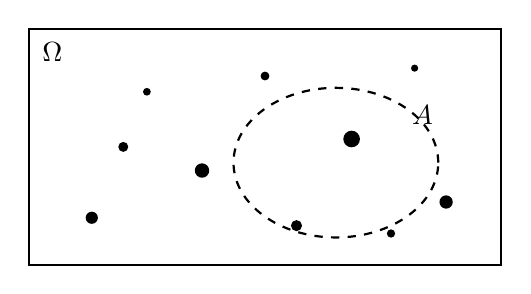
\begin{tikzpicture}
  \draw[thick] (0,0) rectangle (6,3);
  \node at (0.3,2.7) {$\Omega$};
  \foreach \x/\y/\s in {0.8/0.6/2.2, 1.5/2.2/1.4, 2.2/1.2/2.6, 3.0/2.4/1.6, 3.4/0.5/2.0, 4.1/1.6/3.0, 4.9/2.5/1.3, 5.3/0.8/2.4, 1.2/1.5/1.8, 4.6/0.4/1.5}
    \fill (\x,\y) circle (\s pt);
  \draw[thick, dashed] (3.9,1.3) ellipse (1.3 and 0.95);
  \node at (5.0,1.9) {$A$};
\end{tikzpicture}
\caption{A discrete sample space. Each outcome carries a probability weight (dot). The probability of $A$ is the total weight of the outcomes in $A$.}
\label{fig:discrete-sample-space}
\end{figure}

Again, it is up to the modeller to specify these probabilities properly. Fortunately, in many applications all elementary events are equally likely, and thus the probability of each elementary event is 1 divided by the total number of elements in $\Omega$. Because this ``equally likely'' principle is so important, we formulate it as a theorem.

\begin{theorem}[Equilikely principle]\label{thm:equilikely-principle}
If $\Omega$ has a finite number of outcomes, and all are equally likely, then the probability of each event $A$ is
\[
  \Prob(A) = \frac{\abs{A}}{\abs{\Omega}} = \frac{\text{number of elements in } A}{\text{number of elements in } \Omega}.
\]
\end{theorem}

Thus for such sample spaces the calculation of probabilities reduces to counting the number of outcomes in $A$ and $\Omega$ (\cref{sec:counting}).

\begin{example}[Fair die]\label{ex:fair-die}
Consider the experiment where we throw a fair die. How should we define $\Omega$ and $\Prob$? Obviously $\Omega = \set{1, 2, \ldots, 6}$, and common sense shows that we should define $\Prob$ by
\[
  \Prob(A) = \frac{\abs{A}}{6}, \qquad A \subseteq \Omega,
\]
where $\abs{A}$ denotes the number of elements in $A$. For example, the probability of getting an even number is $\Prob(\set{2, 4, 6}) = 3/6 = 1/2$.
\end{example}

\subsection{Continuous sample spaces}\label{sec:continuous-sample-spaces}

When the sample space is not countable, for example $\Omega = \R^{+}$, it is said to be \emph{continuous}.

\begin{example}[Drawing a point in an interval]\label{ex:point-in-interval}
We draw at random a point in the interval $[0, 1]$, each point being equally likely to be drawn. How do we specify the model for this experiment? The sample space is obviously $\Omega = [0, 1]$, which is a continuous sample space. We cannot define $\Prob$ via the elementary events $\set{x}$, $x \in [0, 1]$, because each of these events must have probability 0. However, we can define $\Prob$ as follows: for each $0 \le a \le b \le 1$, let
\[
  \Prob([a, b]) = b - a.
\]
This completely specifies $\Prob$. In particular, the probability that the point falls into any (sufficiently nice) set $A$ is the length of that set.
\end{example}

% ==========================================================================
\section{Counting}\label{sec:counting}
% ==========================================================================

Counting is not always easy. Fortunately, many counting problems can be cast into the simple framework of drawing balls from an urn (\cref{fig:urn}).

\begin{figure}[H]
\centering
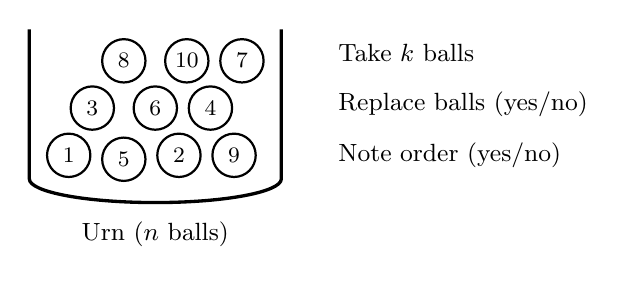
\begin{tikzpicture}
  \draw[very thick] (0,2.2) -- (0,0.3) arc (180:360:1.6 and 0.3) -- (3.2,2.2);
  \foreach \x/\y/\n in {0.5/0.6/1, 1.2/0.55/5, 1.9/0.6/2, 2.6/0.6/9, 0.8/1.2/3, 1.6/1.2/6, 2.3/1.2/4, 1.2/1.8/8, 2.0/1.8/10, 2.7/1.8/7}
    \node[circle, draw, thick, fill=white, inner sep=1pt, minimum size=5.5mm, font=\footnotesize] at (\x,\y) {\n};
  \node[align=left, font=\small, anchor=west] at (3.8,1.9) {Take $k$ balls};
  \node[align=left, font=\small, anchor=west] at (3.8,1.25) {Replace balls (yes/no)};
  \node[align=left, font=\small, anchor=west] at (3.8,0.6) {Note order (yes/no)};
  \node[font=\small] at (1.6,-0.4) {Urn ($n$ balls)};
\end{tikzpicture}
\caption{An urn with $n$ balls.}
\label{fig:urn}
\end{figure}

Consider an urn with $n$ different balls, numbered $1, \ldots, n$, from which $k$ balls are drawn. This can be done in a number of different ways. First, the balls can be drawn one by one, or one could draw all the $k$ balls at the same time. In the first case the order in which the balls are drawn can be noted; in the second case that is not possible. In the latter case we can still assume the balls are drawn one by one, but that the order is not noted. Second, once a ball is drawn, it can either be put back into the urn (after the number is recorded), or left out. This is called, respectively, drawing \emph{with} and \emph{without replacement}. All in all there are 4 possible experiments: (ordered, with replacement), (ordered, without replacement), (unordered, without replacement) and (unordered, with replacement). The art is to recognise a seemingly unrelated counting problem as one of these four urn problems. For example:
\begin{enumerate}
  \item A multiple-choice form has 20 questions, each with 3 choices. Completing the form is drawing 20 balls from an urn containing 3 balls, noting the order, and with replacement.
  \item Betting on the placings (1st, 2nd, 3rd) in a race with 8 horses is drawing 3 balls from an urn containing 8 balls, noting the order, and without replacement.
  \item Choosing 3 of 20 CDs to take to work is drawing 3 balls from an urn containing 20 balls, not noting the order, and without replacement.
  \item A throw of 3 dice is drawing 3 balls from an urn containing 6 balls, not noting the order, and with replacement.
\end{enumerate}
We denote ordered arrangements by vectors, for example $(1, 2, 3) \ne (3, 2, 1)$, and unordered arrangements by sets, for example $\set{1, 2, 3} = \set{3, 2, 1}$. For each of the four cases we consider how the counting works for $n = 4$ and $k = 3$, and then state the general situation.

\subsection{Ordered, with replacement}\label{sec:count-ordered-with}

Here, after we draw each ball, we note the number on the ball and put the ball back. For $n = 4$, $k = 3$, some possible outcomes are $(1,1,1)$, $(4,1,2)$, $(2,3,2)$, $(4,2,1)$, \ldots. To count how many such arrangements there are, we can reason as follows: we have three positions $(\cdot, \cdot, \cdot)$ to fill. Each position can have the numbers 1, 2, 3 or 4, so the total number of possibilities is $4 \times 4 \times 4 = 4^3 = 64$. This is illustrated by the tree diagram in \cref{fig:tree-with-duplication}.

\begin{figure}[H]
\centering
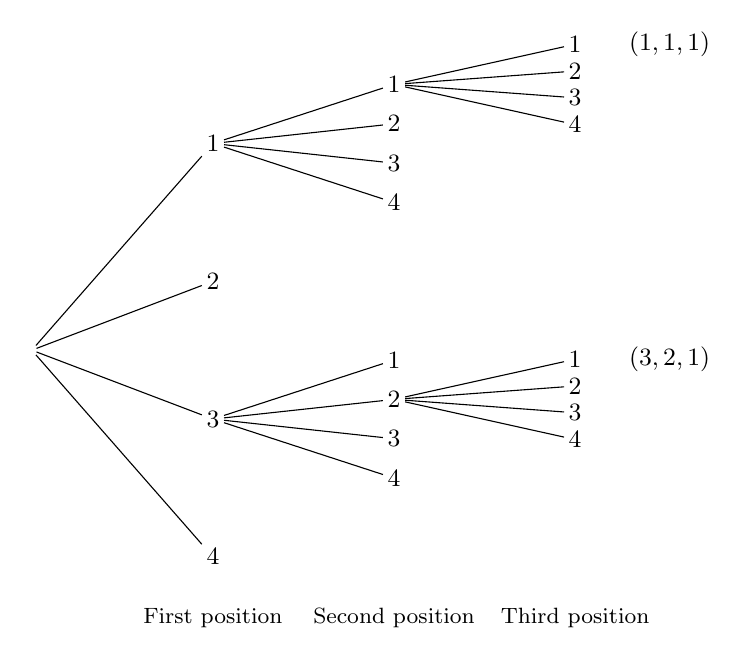
\begin{tikzpicture}[grow=right, level distance=2.3cm, font=\small,
  level 1/.style={sibling distance=1.75cm}, level 2/.style={sibling distance=0.5cm}, level 3/.style={sibling distance=0.34cm},
  every node/.style={inner sep=1.5pt}]
  \node {}
    child {node {4}}
    child {node {3}
      child {node {4}} child {node {3}}
      child {node {2} child {node {4}} child {node {3}} child {node {2}} child {node {1} child[grow=right, level distance=1.2cm] {node {$(3,2,1)$} edge from parent[draw=none]}}}
      child {node {1}}}
    child {node {2}}
    child {node {1}
      child {node {4}} child {node {3}} child {node {2}}
      child {node {1} child {node {4}} child {node {3}} child {node {2}} child {node {1} child[grow=right, level distance=1.2cm] {node {$(1,1,1)$} edge from parent[draw=none]}}}};
  \node[font=\footnotesize] at (2.3,-3.4) {First position};
  \node[font=\footnotesize] at (4.6,-3.4) {Second position};
  \node[font=\footnotesize] at (6.9,-3.4) {Third position};
\end{tikzpicture}
\caption{Part of the tree of ordered arrangements of 3 numbers from $\set{1, 2, 3, 4}$ with repetition allowed. Each first-level node has 4 children, and so on: 64 leaves in all.}
\label{fig:tree-with-duplication}
\end{figure}

\begin{theorem}[Arrangements with order and replacement]\label{thm:count-ordered-with-replacement}
The number of ordered arrangements of $k$ numbers chosen from $\set{1, \ldots, n}$, with replacement (repetition), is $n^k$.
\end{theorem}

\subsection{Ordered, without replacement}\label{sec:count-ordered-without}

Here we again draw $k$ numbers (balls) from the set $\set{1, 2, \ldots, n}$ and note the order, but now we do not replace them. Let $n = 4$ and $k = 3$. Again there are 3 positions to fill $(\cdot, \cdot, \cdot)$, but now the numbers cannot be the same, for example $(1, 4, 2)$ or $(3, 2, 1)$. Such an ordered arrangement is called a \emph{permutation} of size $k$ from the set $\set{1, \ldots, n}$. (A permutation of $\set{1, \ldots, n}$ of size $n$ is simply called a permutation of $\set{1, \ldots, n}$.) For the first position we have 4 possibilities. Once the first position has been chosen, we have only 3 possibilities left for the second position, and after the first two positions have been chosen there are 2 left. So the number of arrangements is $4 \times 3 \times 2 = 24$, as illustrated in \cref{fig:tree-without-duplication}: it is the same tree as in \cref{fig:tree-with-duplication}, but with all ``duplicate'' branches removed.

\begin{figure}[H]
\centering
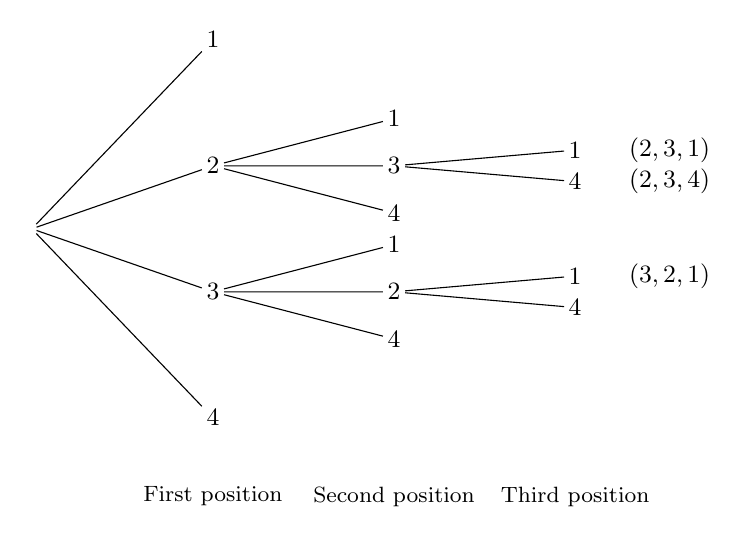
\begin{tikzpicture}[grow=right, level distance=2.3cm, font=\small,
  level 1/.style={sibling distance=1.6cm}, level 2/.style={sibling distance=0.6cm}, level 3/.style={sibling distance=0.4cm},
  every node/.style={inner sep=1.5pt}]
  \node {}
    child {node {4}}
    child {node {3}
      child {node {4}}
      child {node {2} child {node {4}} child {node {1} child[grow=right, level distance=1.2cm] {node {$(3,2,1)$} edge from parent[draw=none]}}}
      child {node {1}}}
    child {node {2}
      child {node {4}}
      child {node {3} child {node {4} child[grow=right, level distance=1.2cm] {node {$(2,3,4)$} edge from parent[draw=none]}} child {node {1} child[grow=right, level distance=1.2cm] {node {$(2,3,1)$} edge from parent[draw=none]}}}
      child {node {1}}}
    child {node {1}};
  \node[font=\footnotesize] at (2.3,-3.4) {First position};
  \node[font=\footnotesize] at (4.6,-3.4) {Second position};
  \node[font=\footnotesize] at (6.9,-3.4) {Third position};
\end{tikzpicture}
\caption{Part of the tree of ordered arrangements of 3 numbers from $\set{1, 2, 3, 4}$ without repetition: 4, then 3, then 2 branches, for 24 leaves in all.}
\label{fig:tree-without-duplication}
\end{figure}

\begin{theorem}[Arrangements with order and without replacement]\label{thm:count-ordered-without-replacement}
The number of permutations of size $k$ from $\set{1, \ldots, n}$ is
\[
  {}^nP_k = n(n-1)\cdots(n-k+1) = \frac{n!}{(n-k)!}.
\]
In particular, when $k = n$, the number of ordered arrangements of $n$ items is $n! = n(n-1)(n-2)\cdots 1$, where $n!$ is called $n$-\emph{factorial}.
\end{theorem}

\subsection{Unordered, without replacement}\label{sec:count-unordered-without}

This time we draw $k$ numbers from $\set{1, \ldots, n}$ but do not replace them (no replication), and do not note the order (so we could draw them in one grab). Taking again $n = 4$ and $k = 3$, a possible outcome is $\set{1, 2, 4}$, $\set{1, 2, 3}$, etc. If we noted the order, there would be ${}^nP_k$ outcomes, amongst which would be $(1,2,4)$, $(1,4,2)$, $(2,1,4)$, $(2,4,1)$, $(4,1,2)$ and $(4,2,1)$. These 6 permutations correspond to the single unordered arrangement $\set{1, 2, 4}$. Such unordered arrangements without replication are called \emph{combinations} of size $k$ from the set $\set{1, \ldots, n}$. To determine the number of combinations of size $k$, we simply need to divide ${}^nP_k$ by the number of permutations of $k$ items, which is $k!$. Thus, in our example ($n = 4$, $k = 3$) there are $24/6 = 4$ possible combinations of size 3.

\begin{theorem}[Arrangements without order and without replacement]\label{thm:count-unordered-without-replacement}
The number of combinations of size $k$ from the set $\set{1, \ldots, n}$ is
\[
  {}^nC_k = \binom{n}{k} = \frac{{}^nP_k}{k!} = \frac{n!}{(n-k)!\,k!}.
\]
\end{theorem}

\subsection{Unordered, with replacement}\label{sec:count-unordered-with}

Taking $n = 4$, $k = 3$, possible outcomes are $\set{3, 3, 4}$, $\set{1, 2, 4}$, $\set{2, 2, 2}$, etc. The trick to solve this counting problem is to represent the outcomes in a different way, via an ordered vector $(x_1, \ldots, x_n)$ representing how many times each element of $\set{1, \ldots, 4}$ occurs. For example, $\set{3, 3, 4}$ corresponds to $(0, 0, 2, 1)$ and $\set{1, 2, 4}$ corresponds to $(1, 1, 0, 1)$. Thus, we can count how many distinct vectors $(x_1, \ldots, x_n)$ there are such that the sum of the components is 3, and each $x_i$ can take the value 0, 1, 2 or 3. Another way of looking at this is to consider placing $k = 3$ balls into $n = 4$ urns, numbered $1, \ldots, 4$. Then $(0, 0, 2, 1)$ means that the third urn has 2 balls and the fourth urn has 1 ball. One way to distribute the balls over the urns is to distribute $n - 1 = 3$ ``separators'' and $k = 3$ balls over $n - 1 + k = 6$ positions, as in \cref{fig:separators}.

\begin{figure}[H]
\centering
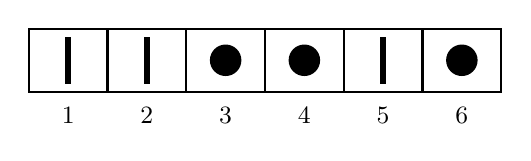
\begin{tikzpicture}
  \foreach \i in {1,...,6} { \draw[thick] (\i-1,0) rectangle (\i,0.8); \node[font=\small] at (\i-0.5,-0.3) {\i}; }
  \foreach \i in {1,2,5} \draw[line width=2pt] (\i-0.5,0.1) -- (\i-0.5,0.7);
  \foreach \i in {3,4,6} \fill (\i-0.5,0.4) circle (0.2);
\end{tikzpicture}
\caption{Distributing $k = 3$ balls over $n = 4$ urns using $n - 1 = 3$ separators in $6$ positions. This arrangement corresponds to $(0, 0, 2, 1)$, that is, to the outcome $\set{3, 3, 4}$.}
\label{fig:separators}
\end{figure}

The number of ways this can be done is equal to the number of ways $k$ positions for the balls can be chosen out of $n - 1 + k$ positions, that is, $\binom{n+k-1}{k}$.

\begin{theorem}[Arrangements without order and with replacement]\label{thm:count-unordered-with-replacement}
The number of different sets $\set{x_1, \ldots, x_k}$ with $x_i \in \set{1, \ldots, n}$, $i = 1, \ldots, k$, is
\[
  \binom{n + k - 1}{k}.
\]
\end{theorem}

\subsection{Summary}\label{sec:counting-summary}

The urn framework is analogous to putting $k$ balls into $n$ bins. The four cases are summarised below.
\begin{center}
\begin{tabular}{@{}lll@{}}
\toprule
Urn: draw $k$ of $n$ balls & Bins: put $k$ balls in $n$ bins & Number of ways \\
\midrule
ordered, with replacement & balls differ, no limit per bin & $n^k$ \\
ordered, without replacement & balls differ, at most 1 per bin & ${}^nP_k$ \\
unordered, without replacement & balls identical, at most 1 per bin & $\binom{n}{k}$ \\
unordered, with replacement & balls identical, no limit per bin & $\binom{n+k-1}{k}$ \\
\bottomrule
\end{tabular}
\end{center}

Returning to our original four problems, we can now solve them easily:
\begin{enumerate}
  \item The total number of ways the exam can be completed is $3^{20} = 3\,486\,784\,401$.
  \item The number of placings is ${}^8P_3 = 336$.
  \item The number of possible combinations of CDs is $\binom{20}{3} = 1140$.
  \item The number of different throws with three dice is $\binom{8}{3} = 56$.
\end{enumerate}

\begin{example}[Tossing a pair of dice]\label{ex:counting-pair-of-dice}
How many outcomes are there when tossing a pair of dice ($n = 6$, $k = 2$)? This depends on whether the dice can be told apart (ordered) and whether repeated values are allowed:
\begin{center}
\begin{tabular}{@{}lcc@{}}
\toprule
 & Repeats allowed & Repeats not allowed \\
\midrule
Dice of different colours (ordered) & $6^2 = 36$ & ${}^6P_2 = 30$ \\
Dice of the same colour (unordered) & $\binom{7}{2} = 21$ & $\binom{6}{2} = 15$ \\
\bottomrule
\end{tabular}
\end{center}
\end{example}

\subsection{Probabilities by counting}\label{sec:probabilities-by-counting}

Once we have learned how to count, we can apply the equilikely principle (\cref{thm:equilikely-principle}) to calculate probabilities.

\begin{example}[Birthday problem]\label{ex:birthday-counting}
What is the probability that, out of a group of 40 people, all have different birthdays?
\end{example}

\begin{solution}
Choosing the birthdays is like choosing 40 balls with replacement from an urn containing the balls $1, \ldots, 365$. Thus, our sample space $\Omega$ consists of vectors of length 40, whose components are chosen from $\set{1, \ldots, 365}$. There are $\abs{\Omega} = 365^{40}$ such vectors, and all are equally likely. Let $A$ be the event that all 40 people have different birthdays. Then $\abs{A} = {}^{365}P_{40} = 365!/325!$. It follows that $\Prob(A) = \abs{A}/\abs{\Omega} \approx 0.109$, so not very big!
\end{solution}

\begin{example}[Five heads in ten tosses]\label{ex:five-heads}
What is the probability that in 10 tosses with a fair coin we get exactly 5 heads and 5 tails?
\end{example}

\begin{solution}
Here $\Omega$ consists of vectors of length 10 consisting of 1s (heads) and 0s (tails), so there are $2^{10}$ of them, and all are equally likely. Let $A$ be the event of exactly 5 heads. We must count how many binary vectors there are with exactly five 1s. This is equivalent to determining in how many ways the positions of the five 1s can be chosen out of 10 positions, that is, $\binom{10}{5}$. Consequently, $\Prob(A) = \binom{10}{5}/2^{10} = 252/1024 \approx 0.25$.
\end{solution}

% ==========================================================================
\section{Conditional probability}\label{sec:conditional-probability}
% ==========================================================================

How do probabilities change when we know that some event $B \subseteq \Omega$ has occurred? Then we know that the outcome lies in $B$, so $A$ will occur if and only if $A \cap B$ occurs (\cref{fig:conditional-probability}). The relative chance of $A$ occurring is therefore $\Prob(A \cap B)/\Prob(B)$.

\begin{figure}[H]
\centering
\begin{tikzpicture}
  \draw[thick] (-2.5,-1.4) rectangle (3.5,1.5);
  \node at (-2.2,1.2) {$\Omega$};
  \fill[defcolor, opacity=0.15] (1.2,0) ellipse (1.6 and 1.0);
  \draw[thick] (-0.3,0) ellipse (1.5 and 0.9);
  \draw[thick] (1.2,0) ellipse (1.6 and 1.0);
  \node at (-1.1,0) {$A$};
  \node at (2.2,0) {$B$};
\end{tikzpicture}
\caption{What is the probability that $A$ occurs, given that the outcome is known to lie in $B$?}
\label{fig:conditional-probability}
\end{figure}

\begin{definition}[Conditional probability]\label{def:conditional-probability}
Given a probability space $(\Omega, \mathcal{F}, \Prob)$ and two events $A, B \in \mathcal{F}$ with $\Prob(B) \ne 0$, the \emph{conditional probability of $A$ given $B$} is
\begin{equation}\label{eq:conditional-probability}
  \Prob(A \given B) = \frac{\Prob(A \cap B)}{\Prob(B)}.
\end{equation}
\end{definition}

\begin{proposition}\label{prop:conditional-probability-is-probability}
For fixed $B$ with $\Prob(B) \ne 0$, $\Prob(\cdot \given B)$ satisfies the probability axioms.
\end{proposition}

\begin{proof}
$\Prob(A \given B) = \Prob(A \cap B)/\Prob(B) \ge 0$, since both the numerator and the denominator are non-negative. $\Prob(\Omega \given B) = \Prob(B)/\Prob(B) = 1$. If $A_1, A_2, \ldots$ are disjoint, then so are $A_1 \cap B, A_2 \cap B, \ldots$, so by the sum rule $\Prob\bigl(\bigcup_i A_i \given B\bigr) = \sum_i \Prob(A_i \cap B)/\Prob(B) = \sum_i \Prob(A_i \given B)$.
\end{proof}

\begin{example}[Throwing two dice]\label{ex:two-dice-conditional}
We throw two dice. Given that the sum of the eyes is 10, what is the probability that one 6 is cast?
\end{example}

\begin{solution}
Let $B$ be the event that the sum is 10,
\[
  B = \set{(4,6), (5,5), (6,4)}.
\]
Let $A$ be the event that one 6 is cast,
\[
  A = \set{(1,6), \ldots, (5,6), (6,1), \ldots, (6,5)}.
\]
Then $A \cap B = \set{(4,6), (6,4)}$. Since all elementary events are equally likely,
\[
  \Prob(A \given B) = \frac{2/36}{3/36} = \frac23.
\]
\end{solution}

\begin{example}[Monty Hall problem]\label{ex:monty-hall}
This is a nice application of conditional probability. Consider a quiz in which the final contestant is to choose a prize which is hidden behind one of three curtains (A, B or C). Suppose, without loss of generality, that the contestant chooses curtain A. Now the quiz master (Monty Hall) always opens one of the other curtains: if the prize is behind B, Monty opens C; if the prize is behind C, Monty opens B; and if the prize is behind A, Monty opens B or C with equal probability, for example by tossing a coin (of course the contestant does not see Monty tossing the coin). Suppose, again without loss of generality, that Monty opens curtain B. The contestant is now offered the opportunity to switch to curtain C. Should the contestant stay with the original choice (A) or switch to the other unopened curtain (C)?
\end{example}

\begin{solution}
The sample space consists of 4 possible outcomes: $Ac$, the prize is behind A and Monty opens C; $Ab$, the prize is behind A and Monty opens B; $Bc$, the prize is behind B and Monty opens C; and $Cb$, the prize is behind C and Monty opens B. Let $A$, $B$, $C$ be the events that the prize is behind A, B and C, respectively. Then $A = \set{Ac, Ab}$, $B = \set{Bc}$ and $C = \set{Cb}$ (\cref{fig:monty-hall}).

\begin{figure}[H]
\centering
\begin{tikzpicture}
  \draw[thick] (0,0) rectangle (4,2);
  \draw[thick] (2,0) -- (2,2) (0,1) -- (2,1);
  \node at (1,1.5) {$Ac$ \quad $\tfrac16$};
  \node at (1,0.5) {$Ab$ \quad $\tfrac16$};
  \draw[thick] (2,1) -- (4,1);
  \node at (3,1.5) {$Cb$ \quad $\tfrac13$};
  \node at (3,0.5) {$Bc$ \quad $\tfrac13$};
\end{tikzpicture}
\caption{The sample space for the Monty Hall problem, with the probability of each outcome.}
\label{fig:monty-hall}
\end{figure}

Obviously $\Prob(A) = \Prob(B) = \Prob(C)$, and since $Ac$ and $Ab$ are equally likely, $\Prob(\set{Ab}) = \Prob(\set{Ac}) = 1/6$. Monty opening curtain B means that we have the information that the event $\set{Ab, Cb}$ has occurred. The probability that the prize is behind A, given this event, is therefore
\[
  \Prob(A \given \text{B is opened}) = \frac{\Prob(\set{Ac, Ab} \cap \set{Ab, Cb})}{\Prob(\set{Ab, Cb})} = \frac{\Prob(\set{Ab})}{\Prob(\set{Ab, Cb})} = \frac{1/6}{1/6 + 1/3} = \frac13.
\]
This is what we expected: the fact that Monty opens a curtain does not give us any extra information that the prize is behind A. So one could think that it does not matter whether we switch or not. But what about $\Prob(B \given \text{B is opened})$? Obviously this is 0: opening curtain B means that event B cannot occur. It follows that $\Prob(C \given \text{B is opened})$ must be $2/3$, since a conditional probability behaves like any other probability and must satisfy Axiom 2. Indeed,
\[
  \Prob(C \given \text{B is opened}) = \frac{\Prob(\set{Cb} \cap \set{Ab, Cb})}{\Prob(\set{Ab, Cb})} = \frac{1/3}{1/6 + 1/3} = \frac23.
\]
Hence, given that B is opened, it is twice as likely that the prize is behind C than behind A. Thus the contestant should switch!
\end{solution}

\subsection{The product rule}\label{sec:product-rule}

By the definition of conditional probability we have
\begin{equation}\label{eq:product-rule-two}
  \Prob(A \cap B) = \Prob(A)\,\Prob(B \given A).
\end{equation}
We can generalise this to $n$ intersections $A_1 \cap A_2 \cap \cdots \cap A_n$, which we abbreviate as $A_1 A_2 \cdots A_n$. This gives the \emph{product rule} of probability, also called the chain rule.

\begin{theorem}[Product rule]\label{thm:product-rule}
Let $A_1, \ldots, A_n$ be a sequence of events with $\Prob(A_1 \cdots A_{n-1}) > 0$. Then
\begin{equation}\label{eq:product-rule}
  \Prob(A_1 \cdots A_n) = \Prob(A_1)\,\Prob(A_2 \given A_1)\,\Prob(A_3 \given A_1 A_2) \cdots \Prob(A_n \given A_1 \cdots A_{n-1}).
\end{equation}
\end{theorem}

\begin{proof}
We only show the proof for 3 events, since the case $n > 3$ follows similarly. By applying \eqref{eq:conditional-probability} to $\Prob(B \given A)$ and $\Prob(C \given A \cap B)$, the right-hand side of \eqref{eq:product-rule} becomes
\[
  \Prob(A)\,\Prob(B \given A)\,\Prob(C \given A \cap B) = \Prob(A)\,\frac{\Prob(A \cap B)}{\Prob(A)}\,\frac{\Prob(A \cap B \cap C)}{\Prob(A \cap B)} = \Prob(A \cap B \cap C),
\]
which is equal to the left-hand side.
\end{proof}

\begin{example}[Birthday problem, via the product rule]\label{ex:birthday-product-rule}
In \cref{ex:birthday-counting} we derived by counting that the probability that all people in a group of 40 have different birthdays is
\begin{equation}\label{eq:birthday-40}
  \frac{365 \times 364 \times \cdots \times 326}{365 \times 365 \times \cdots \times 365} \approx 0.109.
\end{equation}
We can also derive this via the product rule. Let $A_i$ be the event that the first $i$ people have different birthdays, $i = 1, 2, \ldots$. Note that $A_1 \supseteq A_2 \supseteq A_3 \supseteq \cdots$. Therefore $A_n = A_1 \cap A_2 \cap \cdots \cap A_n$, and thus by the product rule
\[
  \Prob(A_{40}) = \Prob(A_1)\,\Prob(A_2 \given A_1)\,\Prob(A_3 \given A_2) \cdots \Prob(A_{40} \given A_{39}).
\]
Now $\Prob(A_k \given A_{k-1}) = (365 - k + 1)/365$, because given that the first $k - 1$ people have different birthdays, there are no duplicate birthdays if and only if the birthday of the $k$th person is chosen from the $365 - (k - 1)$ remaining birthdays. Thus we obtain \eqref{eq:birthday-40}. More generally, the probability that $n$ randomly selected people have different birthdays is
\[
  \Prob(A_n) = \frac{365}{365} \times \frac{364}{365} \times \frac{363}{365} \times \cdots \times \frac{365 - n + 1}{365}, \qquad n \ge 1.
\]
A graph of $\Prob(A_n)$ against $n$ is given in \cref{fig:birthday}. The probability $\Prob(A_n)$ rapidly decreases to zero. Indeed, for $n = 23$ the probability of having no duplicate birthdays is already less than $1/2$.
\end{example}

\begin{figure}[H]
\centering
\begin{tikzpicture}
\begin{axis}[bookplot, xmin=0, xmax=60, ymin=0, ymax=1.05, xlabel={$n$}, ylabel={$\Prob(A_n)$}]
  \addplot[only marks, mark=*, mark size=1pt, color=thmcolor] table[x=n, y=p] {figures/data/birthday.dat};
  \addplot[dashed, thin, domain=0:60] {0.5};
\end{axis}
\end{tikzpicture}
\caption{The probability of having no duplicate birthday in a group of $n$ people, against $n$.}
\label{fig:birthday}
\end{figure}

\begin{example}[Cable matching]\label{ex:cable-matching}
Cables numbered $1, \ldots, n$ on one side are connected to terminals numbered $1, \ldots, n$ on the other side by a random bijection $f \colon \set{1, \ldots, n} \to \set{1, \ldots, n}$, so cable $i$ goes to terminal $f(i)$. The system works if cable $i$ is connected to terminal $i$ for at least one $i$. What is the probability that the system works?
\end{example}

\begin{solution}
Let $E_i$ be the event that cable $i$ is connected properly. We need $\Prob(E_1 \cup E_2 \cup \cdots \cup E_n)$, which by inclusion--exclusion (\cref{thm:inclusion-exclusion}) is
\[
  \sum_i \Prob(E_i) - \sum_{i<j} \Prob(E_i \cap E_j) + \sum_{i<j<k} \Prob(E_i \cap E_j \cap E_k) - \cdots.
\]
Note $\Prob(E_i) = 1/n$. Thus, by the product rule,
\[
  \Prob(E_i \cap E_j) = \Prob(E_i)\,\Prob(E_j \given E_i) = \frac1n \cdot \frac{1}{n-1} \quad (i < j),
\]
\[
  \Prob(E_i \cap E_j \cap E_k) = \frac1n \cdot \frac{1}{n-1} \cdot \frac{1}{n-2} \quad (i < j < k),
\]
and in general
\[
  \sum_{i_1 < \cdots < i_k} \Prob(E_{i_1} \cap \cdots \cap E_{i_k}) = \binom{n}{k} \frac{1}{n(n-1)\cdots(n-k+1)} = \frac{1}{k!},
\]
implying that
\[
  \Prob\Bigl(\bigcup_i E_i\Bigr) = 1 - \frac{1}{2!} + \frac{1}{3!} - \cdots + \frac{(-1)^{n+1}}{n!} = \sum_{i=1}^n \frac{(-1)^{i+1}}{i!} \longrightarrow 1 - \frac1e.
\]
\end{solution}

\subsection{The law of total probability and Bayes' rule}\label{sec:total-probability-bayes}

Suppose $B_1, B_2, \ldots, B_n$ is a \emph{partition} of $\Omega$; that is, $B_1, B_2, \ldots, B_n$ are disjoint and their union is $\Omega$ (\cref{fig:partition}).

\begin{figure}[H]
\centering
\begin{tikzpicture}
  \draw[thick] (0,0) rectangle (6,2.6);
  \draw[thick] (1,0) -- (1.2,2.6) (2,0) -- (2.3,2.6) (3,0) -- (3.1,2.6) (4,0) -- (4.2,2.6) (5,0) -- (4.9,2.6);
  \foreach \x/\i in {0.5/1, 1.6/2, 2.6/3, 3.6/4, 4.6/5, 5.5/6} \node[font=\small] at (\x,2.3) {$B_{\i}$};
  \fill[thmcolor, opacity=0.15] (3,1) ellipse (2.3 and 0.6);
  \draw[thick] (3,1) ellipse (2.3 and 0.6);
  \node at (3,1) {$A$};
  \node at (-0.3,2.4) {$\Omega$};
\end{tikzpicture}
\caption{A partition $B_1, \ldots, B_6$ of the sample space, and an event $A$.}
\label{fig:partition}
\end{figure}

\begin{theorem}[Law of total probability]\label{thm:total-probability}
Let $B_1, \ldots, B_n$ be a partition of $\Omega$ and $A$ an event. Then
\[
  \Prob(A) = \sum_{i=1}^n \Prob(A \given B_i)\,\Prob(B_i).
\]
\end{theorem}

\begin{proof}
By the sum rule, $\Prob(A) = \sum_{i=1}^n \Prob(A \cap B_i)$, and hence, by the definition of conditional probability, $\Prob(A) = \sum_{i=1}^n \Prob(A \given B_i)\,\Prob(B_i)$.
\end{proof}

Combining the law of total probability with the definition of conditional probability gives Bayes' rule.

\begin{theorem}[Bayes' rule]\label{thm:bayes-rule}
Let $B_1, \ldots, B_n$ be a partition of $\Omega$ and $A$ an event. Then
\[
  \Prob(B_j \given A) = \frac{\Prob(B_j \cap A)}{\Prob(A)} = \frac{\Prob(A \given B_j)\,\Prob(B_j)}{\sum_{i=1}^n \Prob(A \given B_i)\,\Prob(B_i)}.
\]
\end{theorem}

A simpler form of Bayes' rule is appropriate in some contexts. It follows directly from the product rule, since $\Prob(A \cap B) = \Prob(A)\,\Prob(B \given A) = \Prob(B)\,\Prob(A \given B)$. Hence
\[
  \Prob(B \given A) = \frac{\Prob(B)\,\Prob(A \given B)}{\Prob(A)}, \qquad \text{provided } \Prob(A) \ne 0.
\]

\begin{example}[Quality control]\label{ex:three-factories}
A company has three factories (1, 2 and 3) that produce the same chip, each producing 15\%, 35\% and 50\% of the total production. The probability of a faulty chip at factory 1, 2, 3 is 0.01, 0.05, 0.02, respectively. Suppose we select randomly a chip from the total production and this chip turns out to be faulty. What is the conditional probability that this chip has been produced in factory 1?
\end{example}

\begin{solution}
Let $B_i$ denote the event that the chip has been produced in factory $i$. The $\set{B_i}$ form a partition of $\Omega$. Let $A$ denote the event that the chip is faulty. We are given that $\Prob(B_1) = 0.15$, $\Prob(B_2) = 0.35$, $\Prob(B_3) = 0.5$, as well as $\Prob(A \given B_1) = 0.01$, $\Prob(A \given B_2) = 0.05$, $\Prob(A \given B_3) = 0.02$. We wish to find $\Prob(B_1 \given A)$, which by Bayes' rule is
\[
  \Prob(B_1 \given A) = \frac{0.15 \times 0.01}{0.15 \times 0.01 + 0.35 \times 0.05 + 0.5 \times 0.02} \approx 0.052.
\]
\end{solution}

% ==========================================================================
\section{Independence}\label{sec:independence}
% ==========================================================================

Independence is a very important concept in probability and statistics. Loosely speaking, it models the lack of information between events. We say $A$ and $B$ are independent if the knowledge that $A$ has occurred does not change the probability that $B$ occurs. That is,
\[
  A, B \text{ independent} \iff \Prob(A \given B) = \Prob(A).
\]
Since $\Prob(A \given B) = \Prob(A \cap B)/\Prob(B)$, an alternative definition of independence is
\[
  A, B \text{ independent} \iff \Prob(A \cap B) = \Prob(A)\,\Prob(B).
\]
This definition also covers the case $B = \emptyset$. We can extend the definition to arbitrarily many events.

\begin{definition}[Independent events]\label{def:independent-events}
The events $A_1, A_2, \ldots$ are said to be \emph{(mutually) independent} if, for any $k$ and any choice of distinct indices $i_1, \ldots, i_k$,
\[
  \Prob(A_{i_1} \cap A_{i_2} \cap \cdots \cap A_{i_k}) = \Prob(A_{i_1})\,\Prob(A_{i_2}) \cdots \Prob(A_{i_k}).
\]
\end{definition}

\begin{remark}[Independence as a model assumption]\label{rem:independence-model-assumption}
In most cases, independence of events is a model assumption. That is, we assume that there exists a $\Prob$ such that certain events are independent.
\end{remark}

\begin{example}[Casting two dice, continued]\label{ex:two-dice-independent}
We cast two fair dice consecutively. Suppose $A$ is the event that the first die is 6 and $B$ is the event that the second one is 6. Then naturally $A$ and $B$ are independent events: knowing that the first die is 6 does not give any information about what the result of the second die will be. Let us check this formally. We have $A = \set{(6,1), (6,2), \ldots, (6,6)}$ and $B = \set{(1,6), (2,6), \ldots, (6,6)}$, so that $A \cap B = \set{(6,6)}$, and
\[
  \Prob(A \given B) = \frac{1/36}{6/36} = \frac16 = \Prob(A).
\]
\end{example}

\subsection{Coin-tossing models}\label{sec:coin-tossing-models}

Independence is the key assumption in the model for repeated coin tosses, from which two important distributions arise.

\begin{example}[A coin toss experiment and the binomial law]\label{ex:binomial-law}
We flip a coin $n$ times. We can write the sample space as the set of binary $n$-tuples:
\[
  \Omega = \set{(0, \ldots, 0), \ldots, (1, \ldots, 1)}.
\]
Here 0 represents tails and 1 represents heads. For example, the outcome $(0, 1, 0, 1, \ldots)$ means that the first throw is tails, the second heads, the third tails, the fourth heads, etc.

How should we define $\Prob$? Let $A_i$ denote the event of heads on the $i$th throw, $i = 1, \ldots, n$. Then $\Prob$ should be such that the events $A_1, \ldots, A_n$ are independent, and moreover $\Prob(A_i)$ should be the same for all $i$. We don't know whether the coin is fair or not, but we can call this probability $p$ ($0 \le p \le 1$). These two rules completely specify $\Prob$. For example, the probability that the first $k$ throws are heads and the last $n - k$ are tails is
\[
  \Prob(\set{(1, 1, \ldots, 1, 0, 0, \ldots, 0)}) = \Prob(A_1) \cdots \Prob(A_k)\,\Prob(A_{k+1}^c) \cdots \Prob(A_n^c) = p^k (1-p)^{n-k}.
\]
Also, let $B_k$ be the event that there are $k$ heads in total. The probability of this event is the sum of the probabilities of the elementary events $\set{(x_1, \ldots, x_n)}$ such that $x_1 + \cdots + x_n = k$. Each of these events has probability $p^k(1-p)^{n-k}$, and there are $\binom{n}{k}$ of them. Thus
\[
  \Prob(B_k) = \binom{n}{k} p^k (1-p)^{n-k}, \qquad k = 0, 1, \ldots, n.
\]
We have thus discovered the \emph{binomial distribution} (\cref{ch:common-distributions}).
\end{example}

\begin{example}[Geometric law]\label{ex:geometric-law}
There is another important law associated with the coin flip experiment. Suppose we flip the coin until heads appears for the first time. Let $C_k$ be the event that heads appears for the first time at the $k$th toss, $k = 1, 2, \ldots$. Then, using the same events $\set{A_i}$ as in \cref{ex:binomial-law}, we can write
\[
  C_k = A_1^c \cap A_2^c \cap \cdots \cap A_{k-1}^c \cap A_k,
\]
so that, with the product rule and the mutual independence of $A_1^c, \ldots, A_{k-1}^c, A_k$, we have the \emph{geometric law}:
\[
  \Prob(C_k) = \Prob(A_1^c) \cdots \Prob(A_{k-1}^c)\,\Prob(A_k) = (1-p)^{k-1} p.
\]
\end{example}
